\section{三角形的五心}
\subsection{五心的定义与性质}
三角形的重心、垂心、内心、外心、旁心称为三角形的五心。


1.重心:三角形的三条中线交于一点,该点叫做三角形的重心;重心将每条中线都分成定比2:1。

$\bigtriangleup{ABC}$中线长度公式:
$$AD^2=\frac{1}{2}\sqrt{2AC^2+2AB^2-BC^2}$$,AD为中线。


2.外心:三角形外接圆的圆心,叫做三角形的外心。



3.垂心:三角形的三条高交于一点,该点叫做三角形的垂心。
\begin{center}
    \includegraphics*[scale=0.75]{8}
\end{center}

垂心的性质:

(1)三角形的三个顶点、三个垂足、垂心这7点可以得到6个四点圆,
三组相似三角形,且$AH\cdot HD=BH\cdot HE=CH\cdot HF$。

(2)H、A、B、C四点中任一点是其余三点为顶点的三角形的垂心,称为一垂心组。

(3)$\angle{BHC}=180^{\circ}-\angle{A}=\angle{B}+\angle{C}$

(4)O是外心,H是垂心,则$\angle{BAO}=\angle{HAC},\angle{ABO}=\angle{HBC}$

(5)H关于三边的对称点在$\bigtriangleup{ABC}$的外接圆上,关于
三边中点的对称点在$\bigtriangleup{ABC}$的外接圆上。

(6)三角形外心O、重心G、垂心H三点共线,且OG:GH=1:2(欧拉线)。

(7)三角形任一顶点到垂心的距离等于外心到对边距离的2倍。

(8)设$\bigtriangleup{ABC}$的垂心为H,外接圆半径为R,
则
$$
\frac{HA}{|\cos{A}|}=\frac{HB}{|\cos{B}|}=\frac{HC}{|\cos{C}|}=2R
$$

(9)三角形的垂心是其垂足三角形的内心。

九点圆:$\bigtriangleup{ABC}$三条高的垂足$D,E,F$,
三边中点$A_1,B_1,C_1$,以及顶点与
垂心H联线段的中点$A_2,B_2,C_2$九点共圆。
\begin{center}
    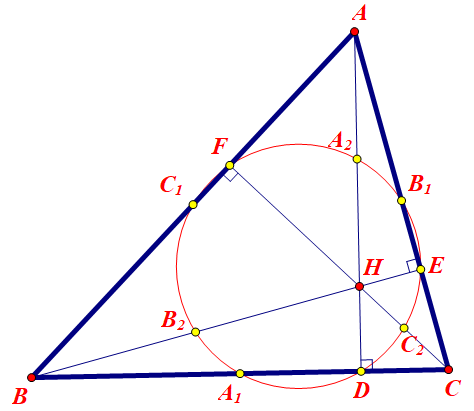
\includegraphics[scale=0.5]{9.png}
\end{center}

证明:
\begin{figure}[H]
    \centering  
    \subfigure{
        \begin{minipage}[t]{0.25\linewidth}
            \centering
            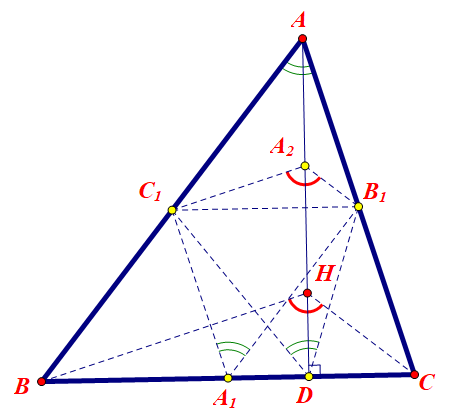
\includegraphics[scale=0.35]{10}
        \end{minipage}}
    \subfigure{
        \begin{minipage}[t]{0.25\linewidth}
            \centering
            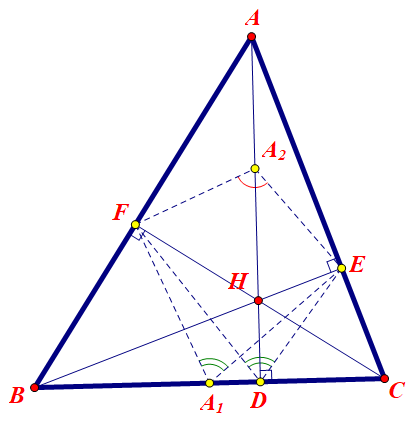
\includegraphics[scale=0.35]{11}
        \end{minipage}}
    \subfigure{
        \begin{minipage}[t]{0.25\linewidth}
            \centering
            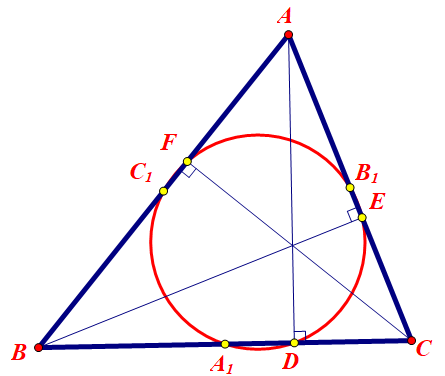
\includegraphics[scale=0.35]{12}
        \end{minipage}}
\end{figure}

位似性质:
\begin{center}
    \includegraphics*[scale=0.75]{13}
\end{center}
\newpage
4.内心:三角形内切圆的圆心,叫做三角形的内心(三角平分线的交点)。

性质:

(1)张角公式:$\angle{BIC}=90^{\circ}+\frac{1}{2}\angle{A}$


(2)设I为$\bigtriangleup ABC$的内心,$AI,BI,CI$分别交外接圆于$D,E,F$,则I为$\bigtriangleup{DEF}$的垂心。
\begin{center}
    \includegraphics*[scale=0.5]{15}
\end{center}

(3)设I为$\bigtriangleup ABC$的内心,$BC=a,AC=b,AB=c$,
$\angle{A}$的平分线交BC于K,交$\bigtriangleup ABC$的外接圆于点D,则
\[
    \frac{AI}{KI}=\frac{DI}{DK}=\frac{AD}{DI}=\frac{b+c}{a}
\]
\begin{center}
    \includegraphics*[scale=0.6]{16}
\end{center}

5.旁心:三角形的旁切圆的圆心,叫做三角形的旁心(三角形一内角平分线和另两顶点处的外角平分线的交点)

(1)鸡爪定理:设$I,I_1$分别是$\bigtriangleup{ABC}$的内心、旁心,延长AI交外接圆于S点,则
$$SI=SB=SC=SI_1$$
\begin{center}
    \includegraphics*[scale=0.5]{17}
\end{center}

(2)三角形的三个旁心与内心构成一垂心组。
\begin{figure}[H]
        \centering  
        \subfigure{
                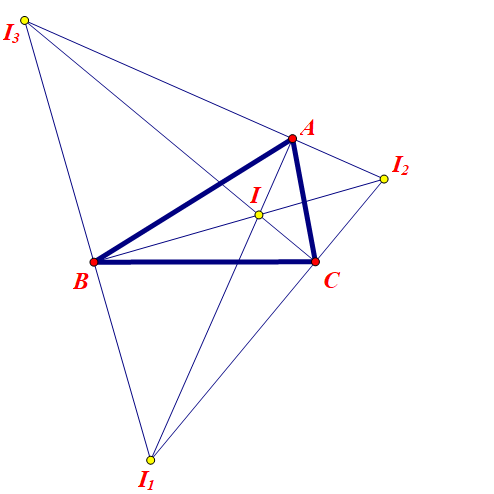
\includegraphics[scale=0.5]{18}}
        \subfigure{
                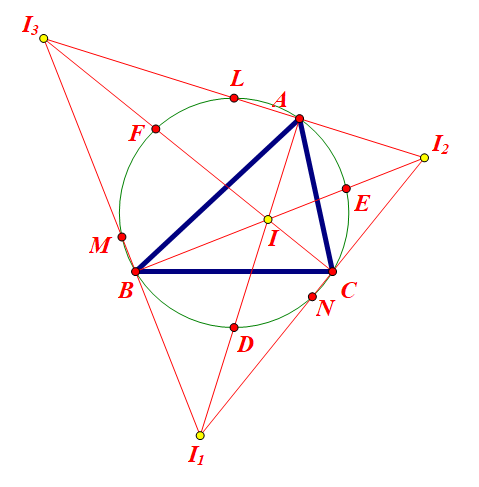
\includegraphics[scale=0.5]{19}}
\end{figure}

\subsection{例题}
1.设H为锐角三角形$\bigtriangleup ABC$的垂心,D为边BC的中点,过点H的直线分别交边AB、AC于点F、E,使得AE=AF,射线DH与$\bigtriangleup ABC$的外接圆交于P.求证:
P、A、E、F四点共圆.

\begin{center}
    \includegraphics*[scale=0.3]{25}
\end{center}

2.设点O是锐角三角形$\bigtriangleup ABC$的外心.分别以$\bigtriangleup ABC$三边的中点为圆心作过点O的圆,这三个圆两两的异于O的交点分别
为K、L、M.证明:点O是$\bigtriangleup KLM$的内心.
\begin{center}
    \includegraphics*[scale=0.3]{26}
\end{center}
\newpage
3.在$\bigtriangleup ABC$中,AB=AC,一个圆内切于$\bigtriangleup ABC$的外接圆$\odot O$于M,并与AB、AC分别相切于P、Q两点.I为线段PQ中点.求证:
I是$\bigtriangleup ABC$的内心.
\begin{center}
    \includegraphics*[scale=0.3]{27}
\end{center}

4.$AD$是直角三角形$ABC$斜边上的高,($AB<AC$),$I_1,I_2$分别是$\bigtriangleup ABD,\bigtriangleup ACD$的内心,$\bigtriangleup AI_1I_2$的外接圆$\odot O$分别交$AB,AC$
于$E,F$,直线$EF,BC$交于点$M$.证明:$I_1,I_2$分别是$\bigtriangleup ODM$的内心与旁心.
\begin{center}
    \includegraphics*[scale=0.4]{28}
\end{center}

5.$\bigtriangleup ABC$的内切圆$I$切$BC,AC$于$D,E$,$K,L$为$AB,AC$中点,证明:$BI,KL,DE$三线共点
\begin{center}
    \includegraphics*[scale=0.4]{29}
\end{center}
\newpage

6.在锐角三角形$ABC$中,$AB<AC$,$O$为外心,$H$为垂心。设直线$AO$与$BC$交于点$D$,点$E$在边BC上且满足$HE // AD$.证明:
$BE=CD$.
\begin{center}
    \includegraphics*[scale=0.4]{30}
\end{center}

7.例题3的推广:

(1)一般情形:设$\odot O'$与$\bigtriangleup ABC$外接圆切于点$D$,与$AB,AC$切于$E,F$点,$I$为线段$EF$中点.证明:$I$为
$\bigtriangleup ABC$的内心.
\begin{center}
    \includegraphics*[scale=0.4]{31}
\end{center}

(2)旁心情形:设$\odot O'$与$\bigtriangleup ABC$外接圆切于点$D$,与$AB,AC$的延长线切于$E,F$点,$I'$为线段$EF$中点.证明:$I'$为
$\bigtriangleup ABC$的$BC$边外的旁心.
\begin{center}
    \includegraphics*[scale=0.4]{32}
\end{center}

8.设$\bigtriangleup ABC$的垂心、外心分别为点$H,O$,BC的中垂线交$\bigtriangleup AOH$的外接圆于$A_1$,
($A_1\neq O$).类似定义点$B_1,C_1$。求证:$AA_1,BB_1,CC_1$三线共点.